\documentclass[a4paper,11pt,twoside]{report}
% KOMPILOWAĆ ZA POMOCĄ pdfLaTeXa, PRZEZ XeLaTeXa MOŻE NIE BYĆ POLSKICH ZNAKÓW

% -------------- Kodowanie znaków, język polski -------------

\usepackage[utf8]{inputenc}
\usepackage[MeX]{polski}
\usepackage[T1]{fontenc}
\usepackage[english,polish]{babel}

\usepackage{subfiles}
\usepackage{graphicx}
\usepackage{caption}
\usepackage{float}
\usepackage{footnote}
\usepackage{multirow}
\usepackage{array}
\usepackage{enumitem}
\usepackage{seqsplit}
\usepackage{longtable}
\raggedbottom
\graphicspath{
    {../screens}
    {../diagrams}
    {../api}
}


\usepackage{amsmath, amsfonts, amsthm, latexsym} % głównie symbole matematyczne, środowiska twierdzeń

\usepackage[final]{pdfpages} % inputowanie pdfa
\usepackage{biblatex}
\addbibresource{links.bib}

\usepackage{commath} % różne komendy ułatwiające pisanie wyrażeń matematycznych --- warto zapoznać się z dokumentacją: https://ctan.gust.org.pl/tex-archive/macros/latex/contrib/commath/commath.pdf

\usepackage[hidelinks]{hyperref} % dla hiperlinków, m.in url , odnośników do równań, czy bibliografii --- opcja hideboxes usuwa prostokąty wokół kiperlinków

% ---------------- Marginesy, akapity, interlinia ------------------

\usepackage[inner=20mm, outer=20mm, bindingoffset=10mm, top=25mm, bottom=25mm]{geometry}


\linespread{1.5}
\allowdisplaybreaks

\usepackage{indentfirst} % opcjonalnie; pierwszy akapit z wcięciem
\setlength{\parindent}{5mm}


%--------------------------- ŻYWA PAGINA ------------------------

\usepackage{fancyhdr}
\pagestyle{fancy}
\fancyhf{}
% numery stron: lewa do lewego, prawa do prawego
\fancyfoot[LE,RO]{\thepage}
% prawa pagina: zawartość \rightmark do lewego, wewnętrznego (marginesu)
\fancyhead[LO]{\sc \nouppercase{\rightmark}}
% lewa pagina: zawartość \leftmark do prawego, wewnętrznego (marginesu)
\fancyhead[RE]{\sc \leftmark}

\renewcommand{\chaptermark}[1]{
\markboth{\thechapter.\ #1}{}}

% kreski oddzielające paginy (górną i dolną):
\renewcommand{\headrulewidth}{0 pt} % 0 - nie ma, 0.5 - jest linia


\fancypagestyle{plain}{% to definiuje wygląd pierwszej strony nowego rozdziału - obecnie tylko numeracja
  \fancyhf{}%
  \fancyfoot[LE,RO]{\thepage}%

  \renewcommand{\headrulewidth}{0pt}% Line at the header invisible
  \renewcommand{\footrulewidth}{0.0pt}
}



% ---------------- Nagłówki rozdziałów ---------------------

\usepackage{titlesec}
\titleformat{\chapter}%[display]
  {\normalfont\Large \bfseries}
  {\thechapter.}{1ex}{\Large}

\titleformat{\section}
  {\normalfont\large\bfseries}
  {\thesection.}{1ex}{}
\titlespacing{\section}{0pt}{30pt}{20pt}
%\titlespacing{\co}{akapit}{ile przed}{ile po}

\titleformat{\subsection}
  {\normalfont \bfseries}
  {\thesubsection.}{1ex}{}


% ----------------------- Spis treści ---------------------------
\def\cleardoublepage{\clearpage\if@twoside
\ifodd\c@page\else\hbox{}\thispagestyle{empty}\newpage
\if@twocolumn\hbox{}\newpage\fi\fi\fi}


% kropki dla chapterów
\usepackage{etoolbox}
\makeatletter
\patchcmd{\l@chapter}
  {\hfil}
  {\leaders\hbox{\normalfont$\m@th\mkern \@dotsep mu\hbox{.}\mkern \@dotsep mu$}\hfill}
  {}{}
\makeatother

\usepackage{titletoc}
\makeatletter
\titlecontents{chapter}% <section-type>
  [0pt]% <left>
  {}% <above-code>
  {\bfseries \thecontentslabel.\quad}% <numbered-entry-format>
  {\bfseries}% <numberless-entry-format>
  {\bfseries\leaders\hbox{\normalfont$\m@th\mkern \@dotsep mu\hbox{.}\mkern \@dotsep mu$}\hfill\contentspage}% <filler-page-format>

\titlecontents{section}
  [1em]
  {}
  {\thecontentslabel.\quad}
  {}
  {\leaders\hbox{\normalfont$\m@th\mkern \@dotsep mu\hbox{.}\mkern \@dotsep mu$}\hfill\contentspage}

\titlecontents{subsection}
  [2em]
  {}
  {\thecontentslabel.\quad}
  {}
  {\leaders\hbox{\normalfont$\m@th\mkern \@dotsep mu\hbox{.}\mkern \@dotsep mu$}\hfill\contentspage}
\makeatother



% ---------------------- Spisy tabel i obrazków ----------------------

\renewcommand*{\thetable}{\arabic{chapter}.\arabic{table}}
\renewcommand*{\thefigure}{\arabic{chapter}.\arabic{figure}}
%\let\c@table\c@figure % jeśli włączone, numeruje tabele i obrazki razem


% --------------------- Definicje, twierdzenia etc. ---------------


% \makeatletter
% \newtheoremstyle{definition}%    % Name
% {3ex}%                          % Space above
% {3ex}%                          % Space below
% {\upshape}%                      % Body font
% {}%                              % Indent amount
% {\bfseries}%                     % Theorem head font
% {.}%                             % Punctuation after theorem head
% {.5em}%                            % Space after theorem head, ' ', or \newline
% {\thmname{#1}\thmnumber{ #2}\thmnote{ (#3)}}%  % Theorem head spec (can be left empty, meaning `normal')
% \makeatother

% ----------------------------- POLSKI --------------------------------

% \theoremstyle{definition}
% \newtheorem{theorem}{Twierdzenie}[chapter]
% \newtheorem{lemma}[theorem]{Lemat}
% \newtheorem{example}[theorem]{Przykład}
% \newtheorem{proposition}[theorem]{Stwierdzenie}
% \newtheorem{corollary}[theorem]{Wniosek}
% \newtheorem{definition}[theorem]{Definicja}
% \newtheorem{remark}[theorem]{Uwaga}



% ----------------------------- Dowód -----------------------------

%\makeatletter
%\renewenvironment{proof}[1][\proofname]
%{\par
%  \vspace{-12pt}% remove the space after the theorem
%  \pushQED{\qed}%
%  \normalfont
%  \topsep0pt \partopsep0pt % no space before
%  \trivlist
%  \item[\hskip\labelsep
%        \sc
%    #1\@addpunct{:}]\ignorespaces
%}
%{%
%  \popQED\endtrivlist\@endpefalse
%  \addvspace{20pt} % some space after
%}
%
%\renewcommand{\qedhere}{\hfill \qedsymbol}
%\makeatother





% -------------------------- POCZĄTEK --------------------------


% --------------------- Ustawienia użytkownika ------------------

\newcommand{\tytul}{System do zdalnej pracy w środowisku graficznym wykorzystujący maszyny wirtualne QEMU z akceleracją sprzętową}
\renewcommand{\title}{Environment for remote work with Graphical User Interface using QEMU virtual machines with hardware acceleration}
\newcommand{\type}{inżyniers} % magisters, licencjac
\newcommand{\supervisor}{dr inż. Marek Kozłowski}



\begin{document}
\sloppy


\includepdf[pages=-]{titlepage/titlepage}


% ------------------ STRONA Z PODPISAMI AUTORA/AUTORÓW I PROMOTORA ------------------


\thispagestyle{empty}\newpage
\null

\vfill

\begin{center}
  \begin{tabular}[t]{ccc}

    ............................................. & \hspace*{100pt} & ............................................. \\
    podpis promotora                              & \hspace*{100pt} & podpisy autorów
  \end{tabular}
\end{center}


% ---------------------------- ABSTRAKTY -----------------------------
% W PRACY PO POLSKU, NAJPIERW STRESZCZENIE PL, POTEM ABSTRACT EN
%
%	Streszczenie powinno zajmować 1 stronę, (czcionką 12)
%

{ \fontsize{12}{14} \selectfont
\begin{abstract}

  \begin{center}
    \tytul
  \end{center}

  Celem projektu jest stworzenie systemu do zdalnej pracy, za pomocą zdalnego pulpitu, wykorzystującego maszyny wirtualne. Jednym z głównych wyróżników projektu jest możliwość użycia maszyn z akceleracją sprzętową oraz integracja z zewnętrznym systemem katalogowym.

  Na wstępie projektu przedstawiony został problem wynikający ze zdalnej pracy oraz wizja systemu, który ma go niwelować wraz z wymaganiami, które musi spełniać.
  W następnym rozdziale znajduje się dokładny opis rozwiązania z wyróżnieniem poszczególnych modułów oraz procesów. Zawarte zostały również wykorzystane technologie, instrukcja uruchomienia systemu oraz sposób użytkowania.
  Kolejny rozdział przedstawia analizę rozwiązania skupiającą się na sposobie testowania poprawności działania systemu oraz jego wynikach.
  Zakończenie opisuje ostateczny stan projektu z wyróżnieniem elementów, które naszym zdaniem wyróżniają się gorszą jakością. Wymienione zostały aspekty o widocznych możliwościach rozwoju oraz znane problemy.

  \noindent \textbf{Słowa kluczowe:} maszyny wirtualne, zdalny pulpit, libvirt, chmura, praca zdalna
\end{abstract}
}

\null\thispagestyle{empty}\newpage

{\selectlanguage{english} \fontsize{12}{14} \selectfont
  \begin{abstract}

    \begin{center}
      \title
    \end{center}
    Goal of thesis is to create environment for remote work, using remote desktop, based on virtual machines. One of main traits is ability to use machines with hardware acceleration and integration with external directory system.

    Introduction describes problem addressed by thesis and proposed environment, aiming to ease it. Chapter also contains technical requirements, which the project must fulfil.
    Next chapter describes in detail the designed environment, including created modules and business processes, used technologies and deployment and use instruction.
    Following chapter analyses the created solution focusing on testing operations and fulfillment of requirements.
    Final chapter describes final state of solution with emphasis on components that stand apart in quality. Possible development paths and open problems were presented.

    \noindent \textbf{Keywords:} virtual machines, remote desktop, libvirt, cloud, remote work
  \end{abstract}
}

\null\thispagestyle{empty}\newpage
% --------------------- OŚWIADCZENIA -----------------------------------------

%
%	KONIECZNE JEST ZAŁĄCZENIE WYPEŁNIONEGO SKANU OŚWIADCZENIA O AUTORSTWIE PRACY. SKAN (W FORMACIE PDF) NALEŻY UMIEŚCIĆ W FOLDERZE scans I NAZWAĆ GO, NP.  oswiadczenie_o_autorstwie_pracy.pdf (W PRZYPADKU INNEJ NAZWY, LUB UMIESZCZENIA W INNYM FOLDERZE KONIECZNE JEST ADEKWATNE ZMODYFIKOWANIE ŚCIEŻKI W PONIŻSZEJ KOMENDZIE.
%
%	komenda załączająca oświadczenie o autorstwie pracy
%
% krzysiu
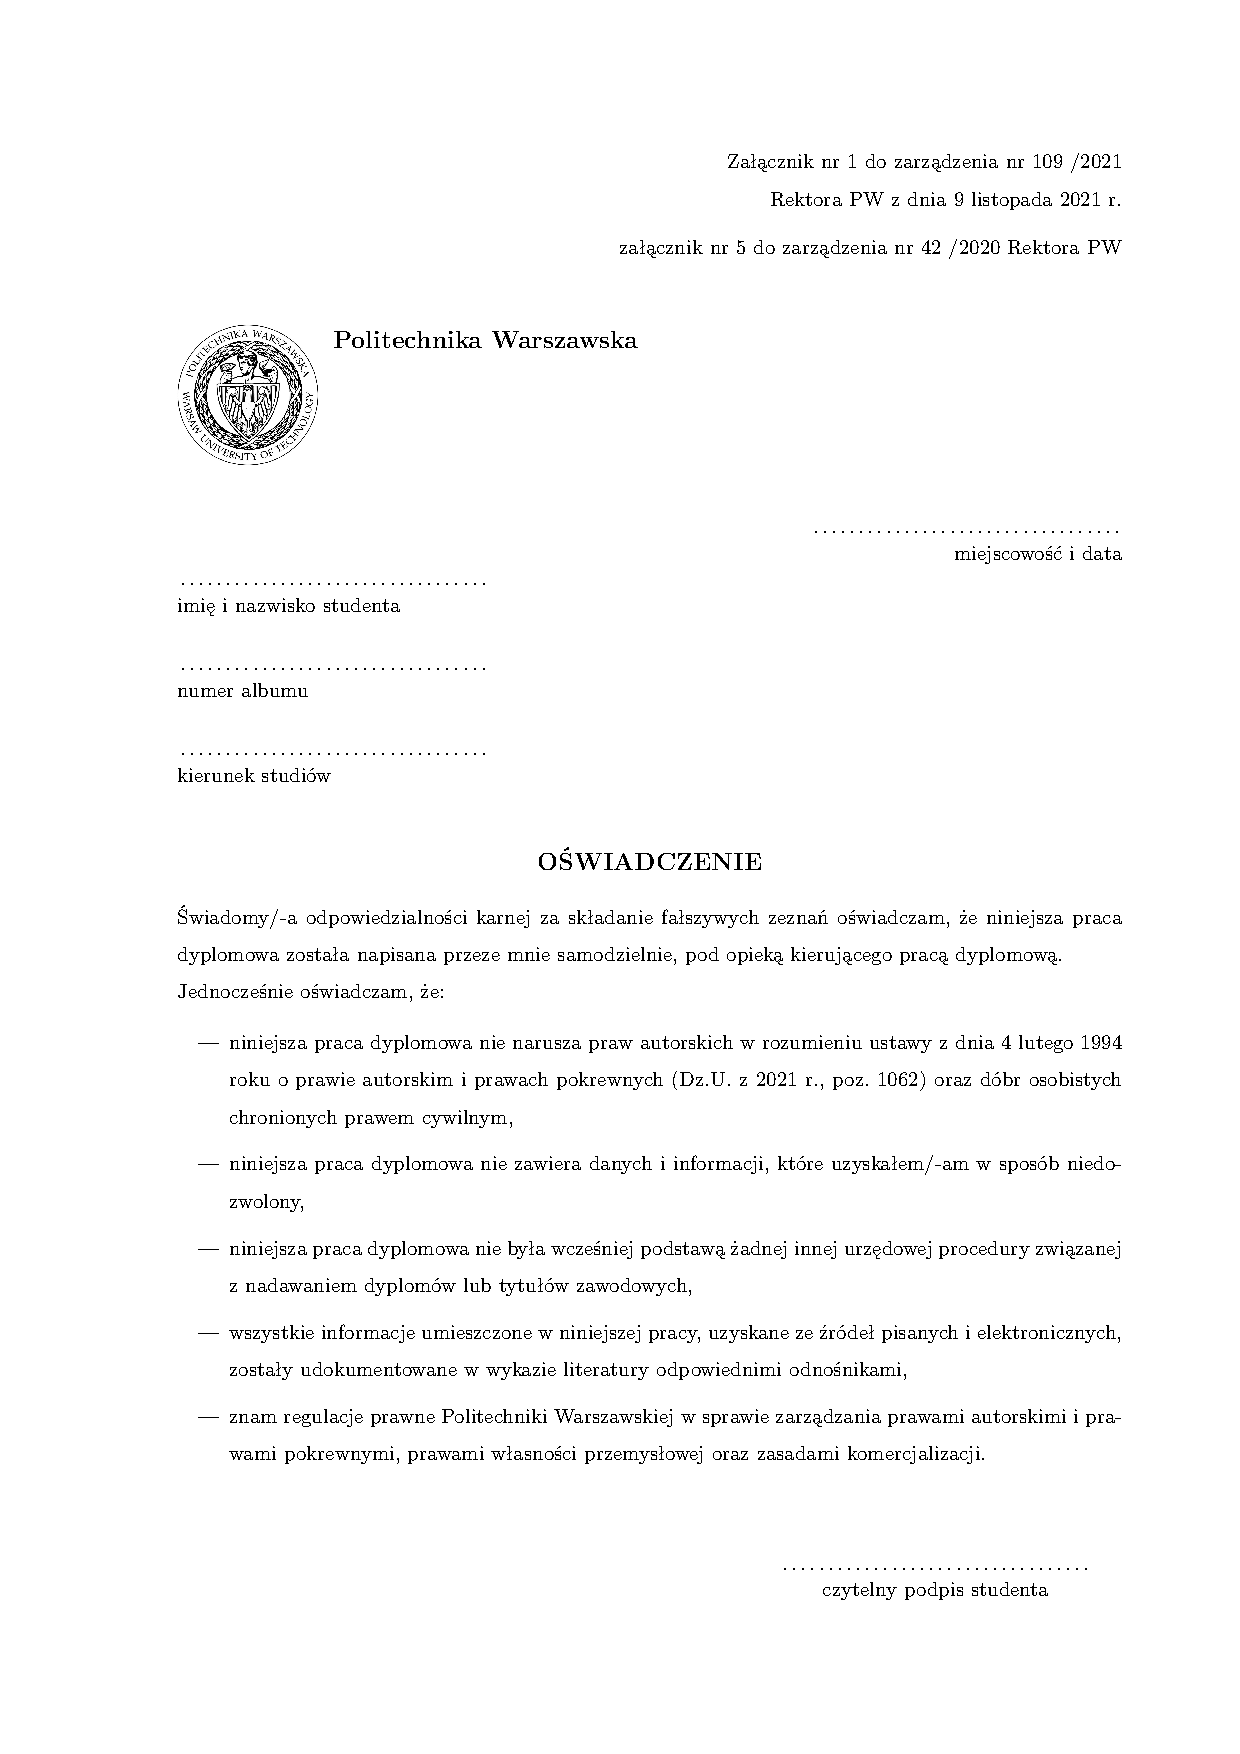
\includepdf[pages=-]{scans/autorstwo-smogork}
\null\thispagestyle{empty}\newpage
% piotrek

\includepdf[pages=-]{scans/autorstwo-widomskip}
\null\thispagestyle{empty}\newpage

% opcjonalne oświadczenie
%
%	komenda załączająca owiadczenie o udzieleniu licencji
%
% krzysiu

\includepdf[pages=-]{scans/licencja-smogork}
\null\thispagestyle{empty}\newpage
% piotrek

\includepdf[pages=-]{scans/licencja-widomskip}
\null\thispagestyle{empty}\newpage

% ------------------- 4. Spis treści ---------------------
\pagenumbering{gobble}
\tableofcontents
\thispagestyle{empty}

\newpage % JEŻELI SPIS TREŚCI MA PARZYSTĄ LICZBĘ STRON, ZAKOMENTOWAĆ
% ALBO JAK KTOŚ WOLI WTEDY DWIE STRONY ODSTĘPU, DODAĆ \null\newpage

% -------------- 5. ZASADNICZA CZĘŚĆ PRACY --------------------
\null\thispagestyle{empty}\newpage
\pagestyle{fancy}
\pagenumbering{arabic}
\setcounter{page}{19} % JEŻELI Z POWODU DUŻEJ ILOŚCI STRON W SPISIE TREŚCI SIĘ NIE ZGADZA, TRZEBA ZMODYFIKOWAĆ RĘCZNIE

\chapter{Wstęp}
% \markboth{}{Wstęp}
% \addcontentsline{toc}{chapter}{Wstęp}
\label{intro}

%Rozdział wstępny
\subfile{sections/wstep.tex}

\chapter{Opis rozwiązania}

%Opis rozwiązania - plan po zrozumieniu problemu
\subfile{sections/opis-rozwiazania.tex}

\chapter{Analiza rozwiązania}
\label{solution-analysis}

%Analiza rozwiązania - analiza wykonanego rozwiązania
\subfile{sections/analiza-rozwiazania.tex}

\chapter{Podsumowanie}
\label{summary}

% Podsymowianie - co osiągneliśmy i co dalej
\subfile{sections/podsumowanie.tex}

% \begin{table}% Koniecznie label po caption, inaczej jest zła numeracja
%   \caption[Opis skrócony]{Opcje dodatkowe dla tabel i rysunków}
%   \label{opcje}
%   \centering
%   \begin{tabular}{|c|p{0.8\textwidth}|}
%     \hline
%     symbol opcji & efekt                                                                                                                                                               \\ \hline
%     \texttt{h}   & bez przemieszczenia, dokładnie w miejscu użycia (uzyteczne w odniesieniu do niewielkich wstawek); raczej niestosowane                                               \\
%     \texttt{t}   & na górze strony; stosowane najczęściej                                                                                                                              \\
%     \texttt{b}   & na dole strony                                                                                                                                                      \\
%     \texttt{p}   & na stronie zawierającej wyłącznie wstawki                                                                                                                           \\
%     \texttt{!}   & ignorując większość parametrów kontrolujacych umieszczanie wstawek, przekroczenie wartosci, których może nie pozwolić na umieszczanie nastepnych wstawek na stronie \\ \hline
%   \end{tabular}
% \end{table}

% W tablicy \ref{opcje} znajdują się opcje dodatkowe otoczeń \texttt{table} i \texttt{figure}.

% \begin{figure}[h!]

%   \begin{center}
%     \setlength{\unitlength}{1mm}

%     \begin{picture}(40, 30)
%       \put(20,1){\line(0,1){20}} % linia

%       % dół
%       \put(20,1){\circle*{2}}
%       \put(25,1){0}

%       % góra
%       \put(20,21){\circle*{2}}
%       \put(25,21){1}
%     \end{picture}

%   \end{center}
%   \caption{Przykładowy rysunek, który można wygenerować w \LaTeX -u}
% \end{figure}

% -------------------- 6. Bibliografia -----------------------
% Bibliografia leksykograficznie wg nazwisk autorów
% Dla ambitnych - można skorzystać z BibTeX-a
\subfile{sections/bibliografia.tex}

\thispagestyle{empty}
\pagenumbering{gobble}


% --- 7. Wykaz symboli i skrótów - jeśli nie ma, zakomentować
% \chapter*{Wykaz symboli i skrótów}

% \begin{tabular}{cl}
%   RDP            & \href{https://docs.microsoft.com/pl-pl/windows/win32/termserv/remote-desktop-protocol?redirectedfrom=MSDN}{Remote Desktop Protocol} \\
%   *              & operator gwiazdka                                                                                                                   \\
%   $\widetilde{}$ & tylda
% \end{tabular}
% \\
% \thispagestyle{empty}


% ----- 8. Spis rysunków - jeśli nie ma, zakomentować --------
\listoffigures
\thispagestyle{empty}


% ------------ 9. Spis tabel - jak wyżej ------------------
\renewcommand{\listtablename}{Spis tabel}
\listoftables
\thispagestyle{empty}


% 10. Spis załączników - jak nie ma załączników, to zakomentować lub usunąć

% \chapter*{Spis załączników}
% \begin{enumerate}
%   \item \texttt{REST\_API\_Overseer.yaml} - dokładna specyfikacja API w standardzie OpenAPI
%         3.0.3
%         %   \item Załącznik 2
%         %   \item Jak nie występują, usunąć rozdział.
% \end{enumerate}
% \thispagestyle{empty}


\end{document}
